\documentclass[conference,6pt]{IEEEtran}
\usepackage[utf8]{inputenc}
\usepackage[T1]{fontenc}
\usepackage{lmodern}
\usepackage[english]{babel}
\usepackage{amsmath, amssymb, mathtools}
\usepackage{graphicx}
\usepackage{xcolor}
\usepackage{hyperref}
\usepackage{algorithm}
\usepackage[noend]{algpseudocode} % noend per non mostrare "end if", "end for", ecc.
\usepackage{booktabs} % Per linee di tabella più professionali
\usepackage{multirow} % Per celle che si estendono su più righe
\usepackage{siunitx}  % Per allineare i numeri per punto decimale e formattazione
\usepackage{enumitem} % Per personalizzare le liste
\usepackage{float}
\usepackage{placeins}
\usepackage{listings}
\usepackage{xcolor}
\usepackage{flushend} 
\usepackage{caption}
\pagenumbering{arabic}



\title{StyCLIP: StyleTransfer in Few-Shot Learning}
\author{
\IEEEauthorblockN{Emanuele Fontana}
\IEEEauthorblockA{
Università degli Studi di Bari Aldo Moro \\
Email: e.fontana7@studenti.uniba.it}
}

\IEEEtitleabstractindextext{%
\begin{abstract}
Few-shot learning for visual artist classification poses a unique challenge due to the diversity of artistic styles and limited labeled data per class. As a baseline, we evaluate the performance of various CLIP-based models on this task. To enhance model generalization, we explore the integration of style transfer techniques directly into the CLIP architecture, hypothesizing that stylization-aware features may better capture artist-specific patterns. However, experimental results on a curated painting dataset show that this approach consistently underperforms compared to standard CLIP variants. Our findings suggest that incorporating style transfer into the model architecture does not yield meaningful gains in artist classification performance under few-shot conditions. The code is available at \url{https://github.com/Fonty02/ComputerVision/tree/main/TIMO}.
\end{abstract}
}%

\newcommand{\Ft}{\mathbf{F}_\text{t}}      % Text features
\newcommand{\Fv}{\mathbf{F}_\text{v}}      % Visual features (support)
\newcommand{\Wt}{\mathbf{W}_\text{t}}      % Text prototypes
\newcommand{\Wv}{\mathbf{W}_\text{v}}      % Visual prototypes (support)
\newcommand{\fv}{\mathbf{f}_\text{v}}      % Query visual feature
\newcommand{\Figt}{\mathbf{F}_\text{IGT}}  % IGT features
\newcommand{\Ftgi}{\mathbf{F}_\text{TGI}}  % TGI features
\newcommand{\R}{\mathbb{R}}

\begin{document}
\footnotesize 
\maketitle

\IEEEdisplaynontitleabstractindextext



\section{Introduction}

Visual artist classification represents a fundamental challenge in computer vision, bridging art history and automated content analysis. The exponential growth of digitized art collections necessitates automated systems to reduce manual effort while democratizing access to art historical knowledge.

We address few-shot learning for artist classification, where models must identify artistic styles using limited labeled examples. This task is particularly challenging as artistic style encompasses subtle visual characteristics like brushstroke patterns, color palettes, and compositional techniques requiring specialized domain knowledge.

While CLIP-based few-shot methods excel at semantic understanding, they may overlook fine-grained stylistic nuances crucial for artist identification. We propose StyCLIP, a novel CLIP extension incorporating artistic style through Gram matrix features. Our contributions include: (1) a StyleAdapter module integrating style-aware features with semantic representations, (2) comprehensive evaluation using a curated ArtGraph dataset subset, and (3) extensive experiments to evaluate the impact of style-aware features on few-shot artist classification.


\section{Related Work}

\subsection{Style Transfer}

Style transfer techniques, pioneered by Gatys et al. \cite{StyleTransfer}, revealed that deep neural networks implicitly encode stylistic information in their intermediate layers. Their seminal work showed that the correlations between feature activations, captured through Gram matrices, effectively represent artistic style independently of content. While originally developed for style transfer applications, Gram matrix representations offer valuable insights into modeling artistic style for classification tasks.

\subsection{Few-Shot Learning and Meta-Learning}
Few-shot learning (FSL) methodologies aim to develop models that can generalize from limited examples, making them particularly relevant for artistic domains where comprehensive datasets are rare. Meta-learning approaches Prototypical Networks \cite{ProtoNet}  fundamentally changed the FSL landscape by learning to learn from small samples.

\subsection{Contrastive Language-Image Pretraining}
The emergence of large-scale vision-language models like CLIP \cite{CLIP} has opened new possibilities for few-shot artistic recognition by leveraging textual descriptions of artistic styles. These models project images and text into a shared embedding space where semantically related concepts are positioned closer together. 


Methods like TIP-Adapter \cite{TipAdapter} incorporate few-shot examples through a non-parametric cache model that complements zero-shot predictions. Other approaches like APE \cite{APE} enhance performance by selectively refining CLIP's features based on adaptive prior refinement, while GDA-CLIP \cite{GDA_CLIP} introduces a novel gradient-based adaptation technique to optimize decision boundaries. More sophisticated approaches like TIMO \cite{TIMO} leverage mutual guidance between text and image modalities to improve low-shot performance.


Our work investigates integrating Gram matrix-based style representations into CLIP architectures to enhance few-shot artist classification performance.

\section{Data}

We utilize a subset of the ArtGraph dataset \cite{ArtGraph}, a comprehensive art knowledge graph containing over 100,000 paintings with metadata. We created two non-overlapping subsets: one for few-shot evaluation and another for StyCLIP training.

\subsection{ArtGraph Few-Shot Subset}

Our few-shot dataset follows a systematic two-stage selection process:

\begin{itemize}
    \item \textbf{Style Selection:} Top 10 artistic styles by artwork count
    \item \textbf{Artist Filtering:} Artists with 30-50 artworks per style (up to 10 artists per style)
\end{itemize}

\textbf{Data Splits:} 80\% support set, 10\% validation, 10\% query set to accommodate varying portfolio sizes.

\subsection{ArtGraph StyCLIP Subset}

For style-aware training, we use complementary artists (16-50 artworks) excluded from the few-shot subset, ensuring no data leakage between training and evaluation phases.
\section{Background: TIMO}

TIMO (Text-Image Mutual Guidance Optimization) is a method proposed to improve training-free Few-Shot Learning with CLIP, specifically designed to address the problems of anomalous visual misalignment and variable quality of textual prompts resulting from independent modality modeling. TIMO introduces a mutual guidance mechanism between text and image, composed of two main branches that work synergistically:

\subsection{Text-Guided Image (TGI)}
This branch uses textual representations to guide and refine visual features, helping to address misalignment issues in the image modality.

The method computes similarity weights between textual prompts and visual prototypes. For each class $i$ with textual prompt $F_{i,p}^t$ and visual prototype $W_i^v$, the similarity weight is:
\[
s_{i,p}^t = \frac{F_{i,p}^t \cdot W_i^v}{||F_{i,p}^t|| ||W_i^v||}
\]

These weights guide the selection of relevant textual prompts. The visual support features $F_v$ are then combined with weighted textual features to create enriched representations:
\[
F_{\text{TGI}} = \text{Concat}(F_v, F^t \odot S, \text{dim}=1)
\]
where $S$ contains the similarity weights and $\odot$ denotes element-wise multiplication. Finally, TGI logits are computed using a classifier built on these enriched features.

\subsection{Image-Guided Text (IGT)}
This branch improves textual prompt quality by leveraging visual representations as guidance, maintaining prompt diversity while enhancing alignment.

For each class $i$, the method finds optimal weights $r_i$ for its textual prompts that maximize alignment with the visual prototype:
\[
\max_{r_i} r_i^T (F_i^t W_i^v) \quad \text{subject to } ||r_i|| = \gamma
\]

The constraint $||r_i|| = \gamma$ preserves prompt diversity. These weights are normalized to obtain a distribution $R$ over prompts. The original textual features are then transformed using these weights to create rectified textual prototypes:
\[
F_{\text{IGT}}[n, d] = \sum_{p=1}^P R[n,p] \cdot F^t[n,p,d]
\]

IGT logits are computed using a classifier built on these rectified features.

\subsection{Combination}
The logits obtained from the two guided branches, $logits_{\text{TGI}}$ and $logits_{\text{IGT}}$, are combined via a weighted sum to produce TIMO's final logits:
\[
\text{logits}_{\text{TIMO}} = \text{logits}_{\text{TGI}} + \alpha \cdot \text{logits}_{\text{IGT}}
\]
The hyperparameter $\alpha$ balances the contribution of the two guided branches and is typically determined through a grid search on a validation set. This combination mechanism allows TIMO to leverage the strengths of both modalities, guiding each other to improve few-shot classification performance.
\section{Our Approach: StyCLIP}

In this section, we describe our approach

\subsection{StyCLIP structure}

StyCLIP extends the standard CLIP architecture by integrating explicit style representations through Gram matrix features, specifically designed to capture artistic style information that complements semantic understanding. 

\subsubsection{Standard CLIP}

The baseline CLIP model consists of:
\begin{itemize}
    \item \textbf{Visual Encoder}: To extract visual features from images into a D-dimensional embedding space
    \item \textbf{Text Encoder}: To extract semantic features from text descriptions into a D-dimensional embedding space
    \item \textbf{Contrastive Learning}: To align visual and text embeddings in a shared space using a contrastive loss function
\end{itemize}

\subsubsection{StyCLIP Architecture Overview}

Our StyCLIP architecture maintains the original CLIP backbone while introducing three key components for style-aware feature learning:
\begin{figure*}[t!]
    \centering
    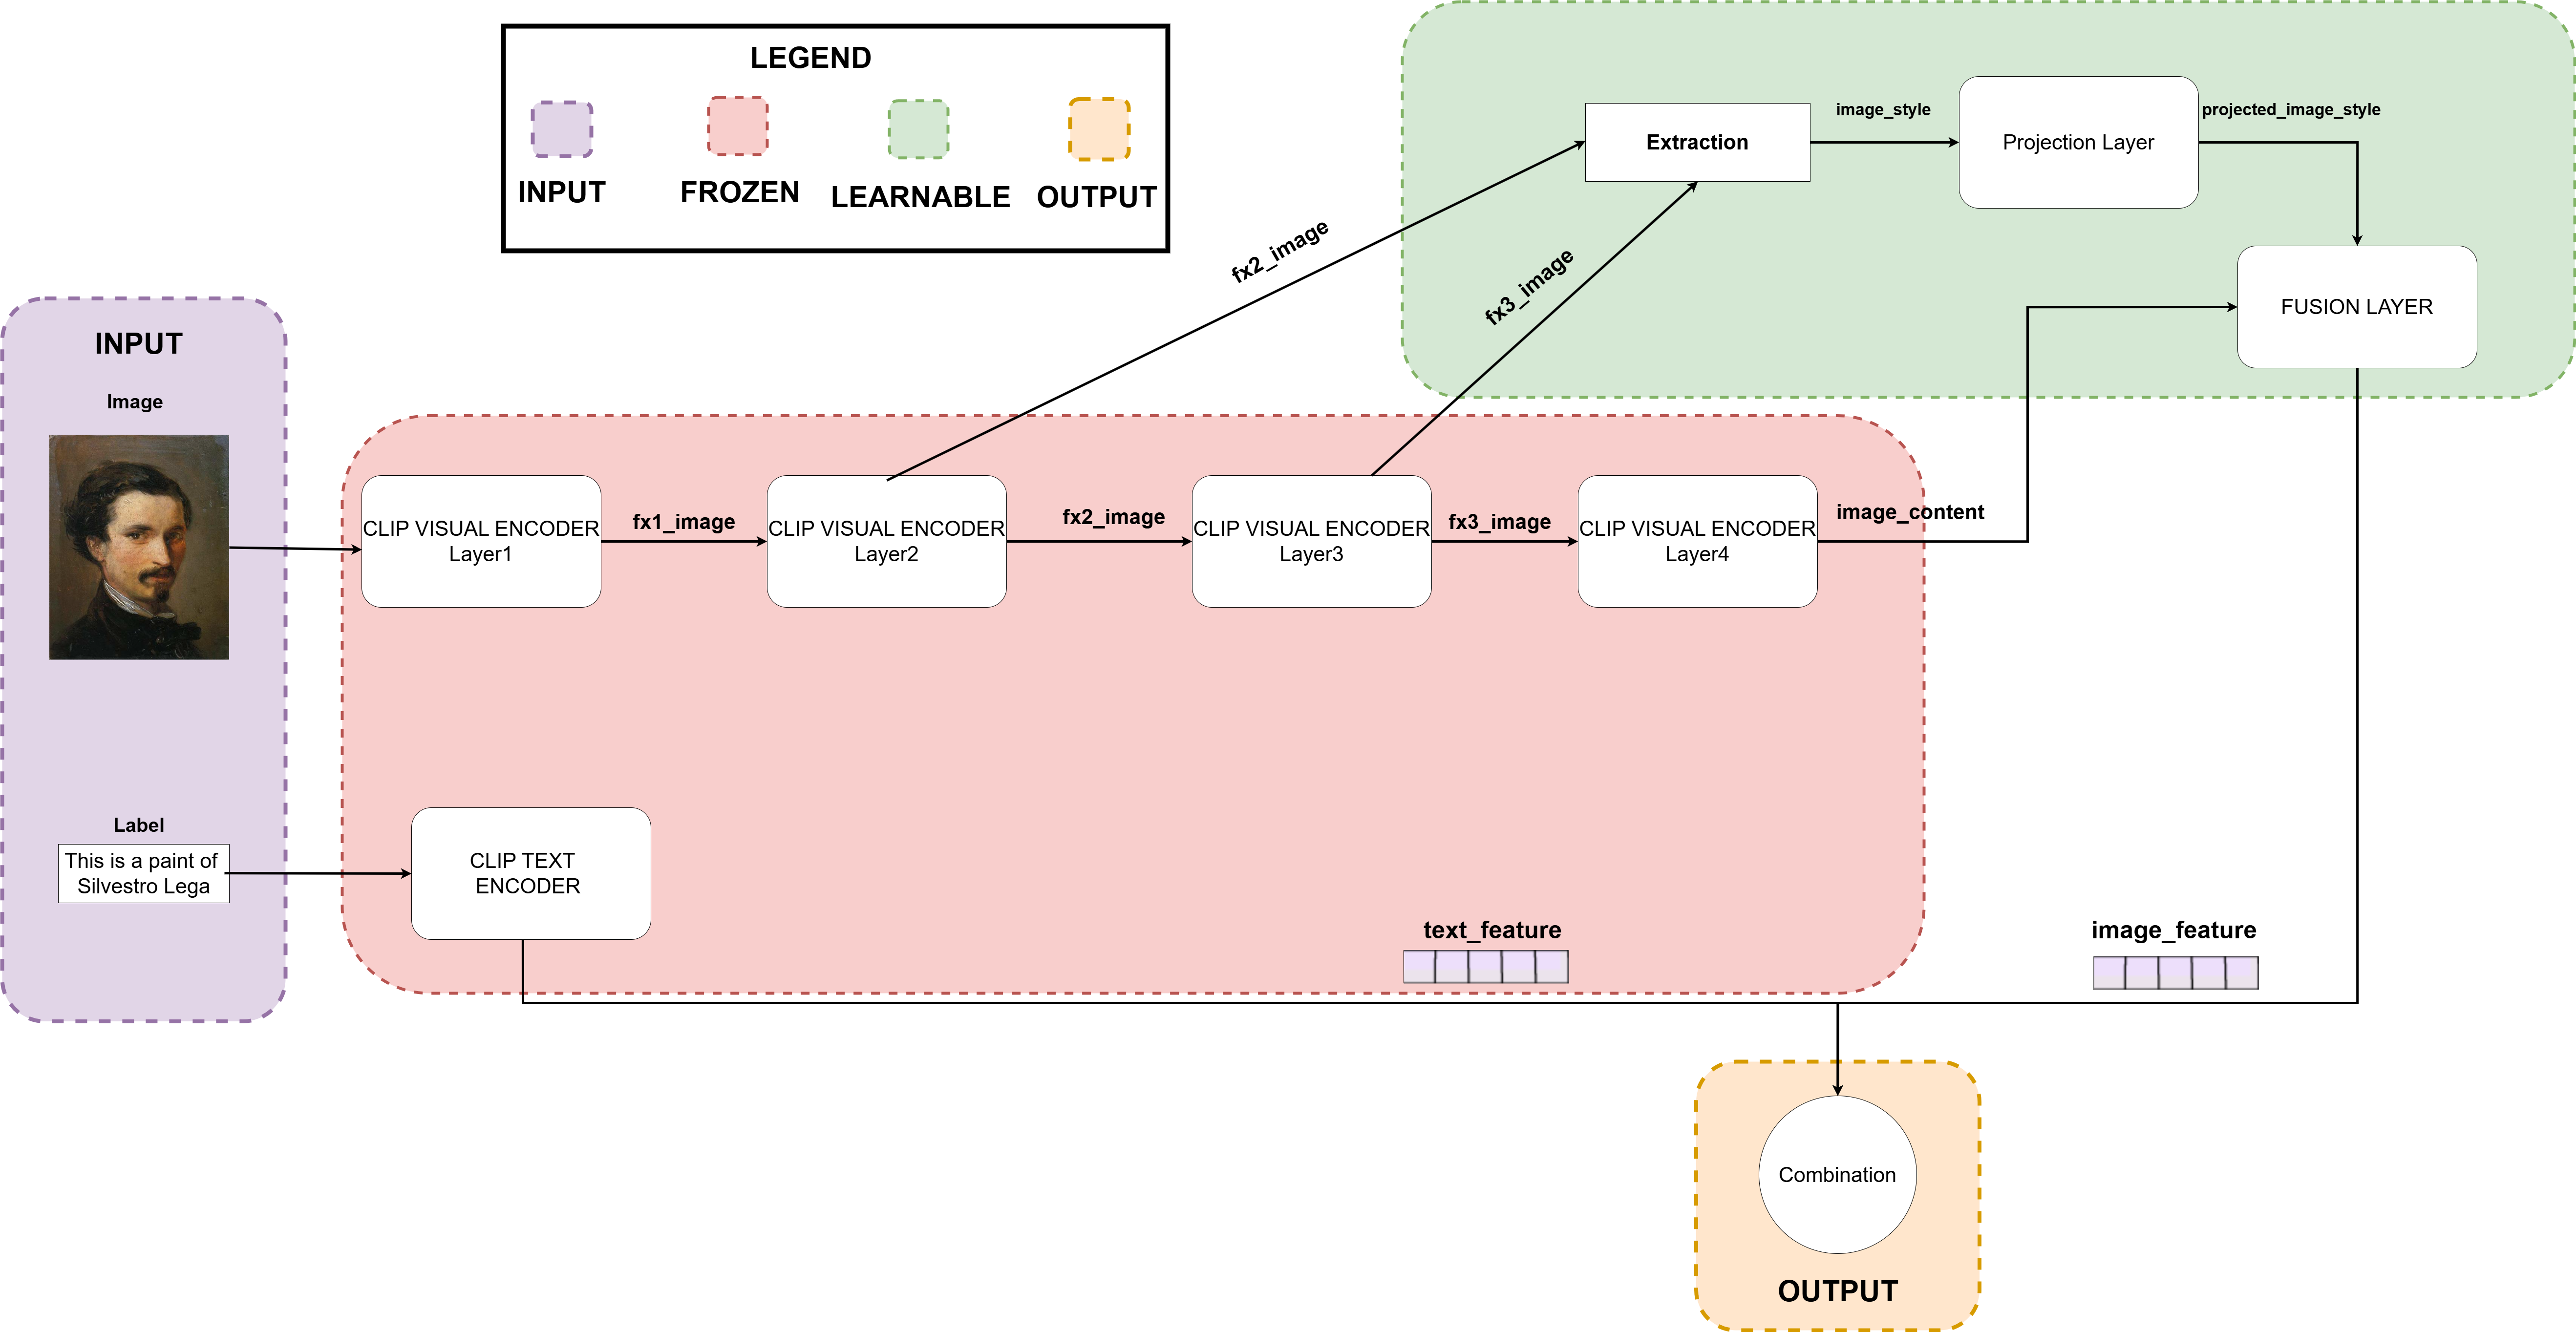
\includegraphics[width=\linewidth,height=0.4\textheight]{../img/StyCLIP.png}
    \caption{StyCLIP Architecture Overview}
\end{figure*}
\begin{itemize}
    \item \textbf{Gram Matrix Extraction Module}: Captures style-specific correlations from intermediate visual features
    \item \textbf{Style Feature Projection Layers}: Dimensionality reduction for Gram matrix representations
    \item \textbf{Fusion Adapter}: Integration of semantic and style features through a bottleneck architecture
\end{itemize}

\paragraph{Gram Matrix Extraction Module}

We extract style-specific correlations from intermediate visual encoder layers using forward hooks registered on ResNet-50 layers. For feature maps $F_l \in \mathbb{R}^{C_l \times H_l \times W_l}$ from layer $l$, we compute the Gram matrix $G_l \in \mathbb{R}^{C_l \times C_l}$ as:

\[
G_l^{(i,j)} = \frac{1}{H_l \times W_l} \sum_{h=1}^{H_l} \sum_{w=1}^{W_l} F_l^{(i,h,w)} \cdot F_l^{(j,h,w)}
\]

where $G_l^{(i,j)}$ represents channel correlations at layer $l$. We extract Gram matrices from multiple ResNet-50 blocks (specifically the second and third residual blocks, corresponding to `layer2` and `layer3` in the ResNet architecture) to capture style information at different abstraction levels. The upper triangular portion of each Gram matrix is vectorized to reduce redundancy.

\paragraph{Style Feature Projection}

Each Gram matrix $G_l$ is flattened and processed through dedicated MLPs with Xavier initialization:

\[
\mathbf{s}_l = \text{MLP}_l(\text{flatten}(\text{triu}(G_l)))
\]

where $\text{triu}(G_l)$ extracts the upper triangular portion to reduce redundancy. The MLP structure follows:

\[
\text{MLP}_l(\mathbf{x}) = \text{Linear}(\mathbf{x})
\]

The projection reduces dimensionality from the vectorized Gram matrix size to a fixed embedding dimension $d_{style}$ per layer, which is then distributed equally among all selected layers.

\paragraph{Fusion Adapter}

The fusion adapter combines semantic features $\mathbf{f}_{sem} \in \mathbb{R}^{d_{clip}}$ from CLIP with style features $\mathbf{s}_{concat} = [\mathbf{s}_{l_1}, ..., \mathbf{s}_{l_k}]$ from Gram matrices through a bottleneck architecture:

\[
\mathbf{f}_{fused} = \mathbf{W}_{down} \cdot [\mathbf{f}_{sem}; \mathbf{s}_{concat}]
\]

\[
\mathbf{f}_{output} = \alpha \cdot \mathbf{W}_{up}(\text{ReLU}(\mathbf{f}_{fused})) + \mathbf{f}_{sem}
\]

where $\alpha$ is a learned scaling factor and the residual connection preserves semantic information while incorporating style-aware features.

\section{Experiments}
In this section, we describe the experimental setup, including hyperparameter tuning, training strategy, and evaluation protocol.
\subsection{StyCLIP hyperparameters tuning and training}
In our case the backbone used for the standard CLIP model is a ResNet-50 (RN50) architecture. The StyCLIP model is trained using a combination of style-aware features extracted from Gram matrices and the standard CLIP architecture.
During training, the CLIP backbone remains frozen while only the style projection layers and fusion adapter are optimized. This approach:
\begin{itemize}
    \item Preserves pre-trained semantic knowledge from CLIP
    \item Reduces computational requirements by limiting trainable parameters
    \item Enables efficient fine-tuning on artistic datasets
    \item Maintains stability in the learned representations
\end{itemize}


StyCLIP hyperparameters are optimized using Optuna \cite{Optuna} with the following search space:

\textbf{Architectural Parameters:} Fusion bottleneck dimension \{64, 128, 256\}; dropout rate [0.0, 0.5, step=0.1]

\textbf{Training Parameters:} Learning rate log-uniform [10\textsuperscript{-5}, 10\textsuperscript{-3}]; weight decay log-uniform [10\textsuperscript{-6}, 10\textsuperscript{-3}]

\subsubsection{Meta-Learning Training Protocol}

Our training employs a prototypical network \cite{ProtoNet} approach adapted for artistic classification:

\textbf{Episodic Training Structure:} Each training episode consists of N-way classification tasks where N=10 artists are randomly sampled. For each artist, we sample K support examples and Q=3 query examples, creating balanced few-shot scenarios.

\textbf{K-Shot Experimental Design:} Our evaluation examines StyCLIP performance across two key support set configurations to understand how training data quantity affects style-aware few-shot learning:

\begin{itemize}
    \item \textbf{1-Shot (K=1):} Minimal data scenario testing generalization from single examples per artist
    \item \textbf{4-Shot (K=4):} Enhanced data setting enabling more robust prototype estimation and style variation capture
\end{itemize}

This comparison reveals how explicit style modeling benefits vary with available training examples.

\subsubsection{Training Configuration}
We employ AdamW optimization with cosine annealing learning rate scheduling. A warmup period of 100 steps ensures stable training initialization. Training incorporates early stopping with patience=10 epochs and minimum improvement threshold of 0.001 to prevent overfitting while maintaining training efficiency. For robust hyperparameter selection, we use a separate meta-validation set comprising 30\% of available artists, ensuring no overlap with training data. Only the newly introduced components (Gram matrix projections and fusion adapter) are trainable. 

\subsubsection{Optimization Strategy}

The Optuna framework enables efficient hyperparameter exploration using Tree-structured Parzen Estimator (TPE) for intelligent sampling, median pruning for early termination of unpromising trials, and 15 trials per K-shot configuration to balance exploration with computational efficiency.

This systematic approach ensures robust hyperparameter selection while maintaining computational feasibility for the K-shot comparative analysis.

\subsection{Evaluation of different models}

We conduct comprehensive experiments to evaluate StyCLIP against established few-shot learning baselines using a systematic evaluation protocol designed to ensure robust and statistically significant results.


\begin{figure*}[t!]
    \centering
    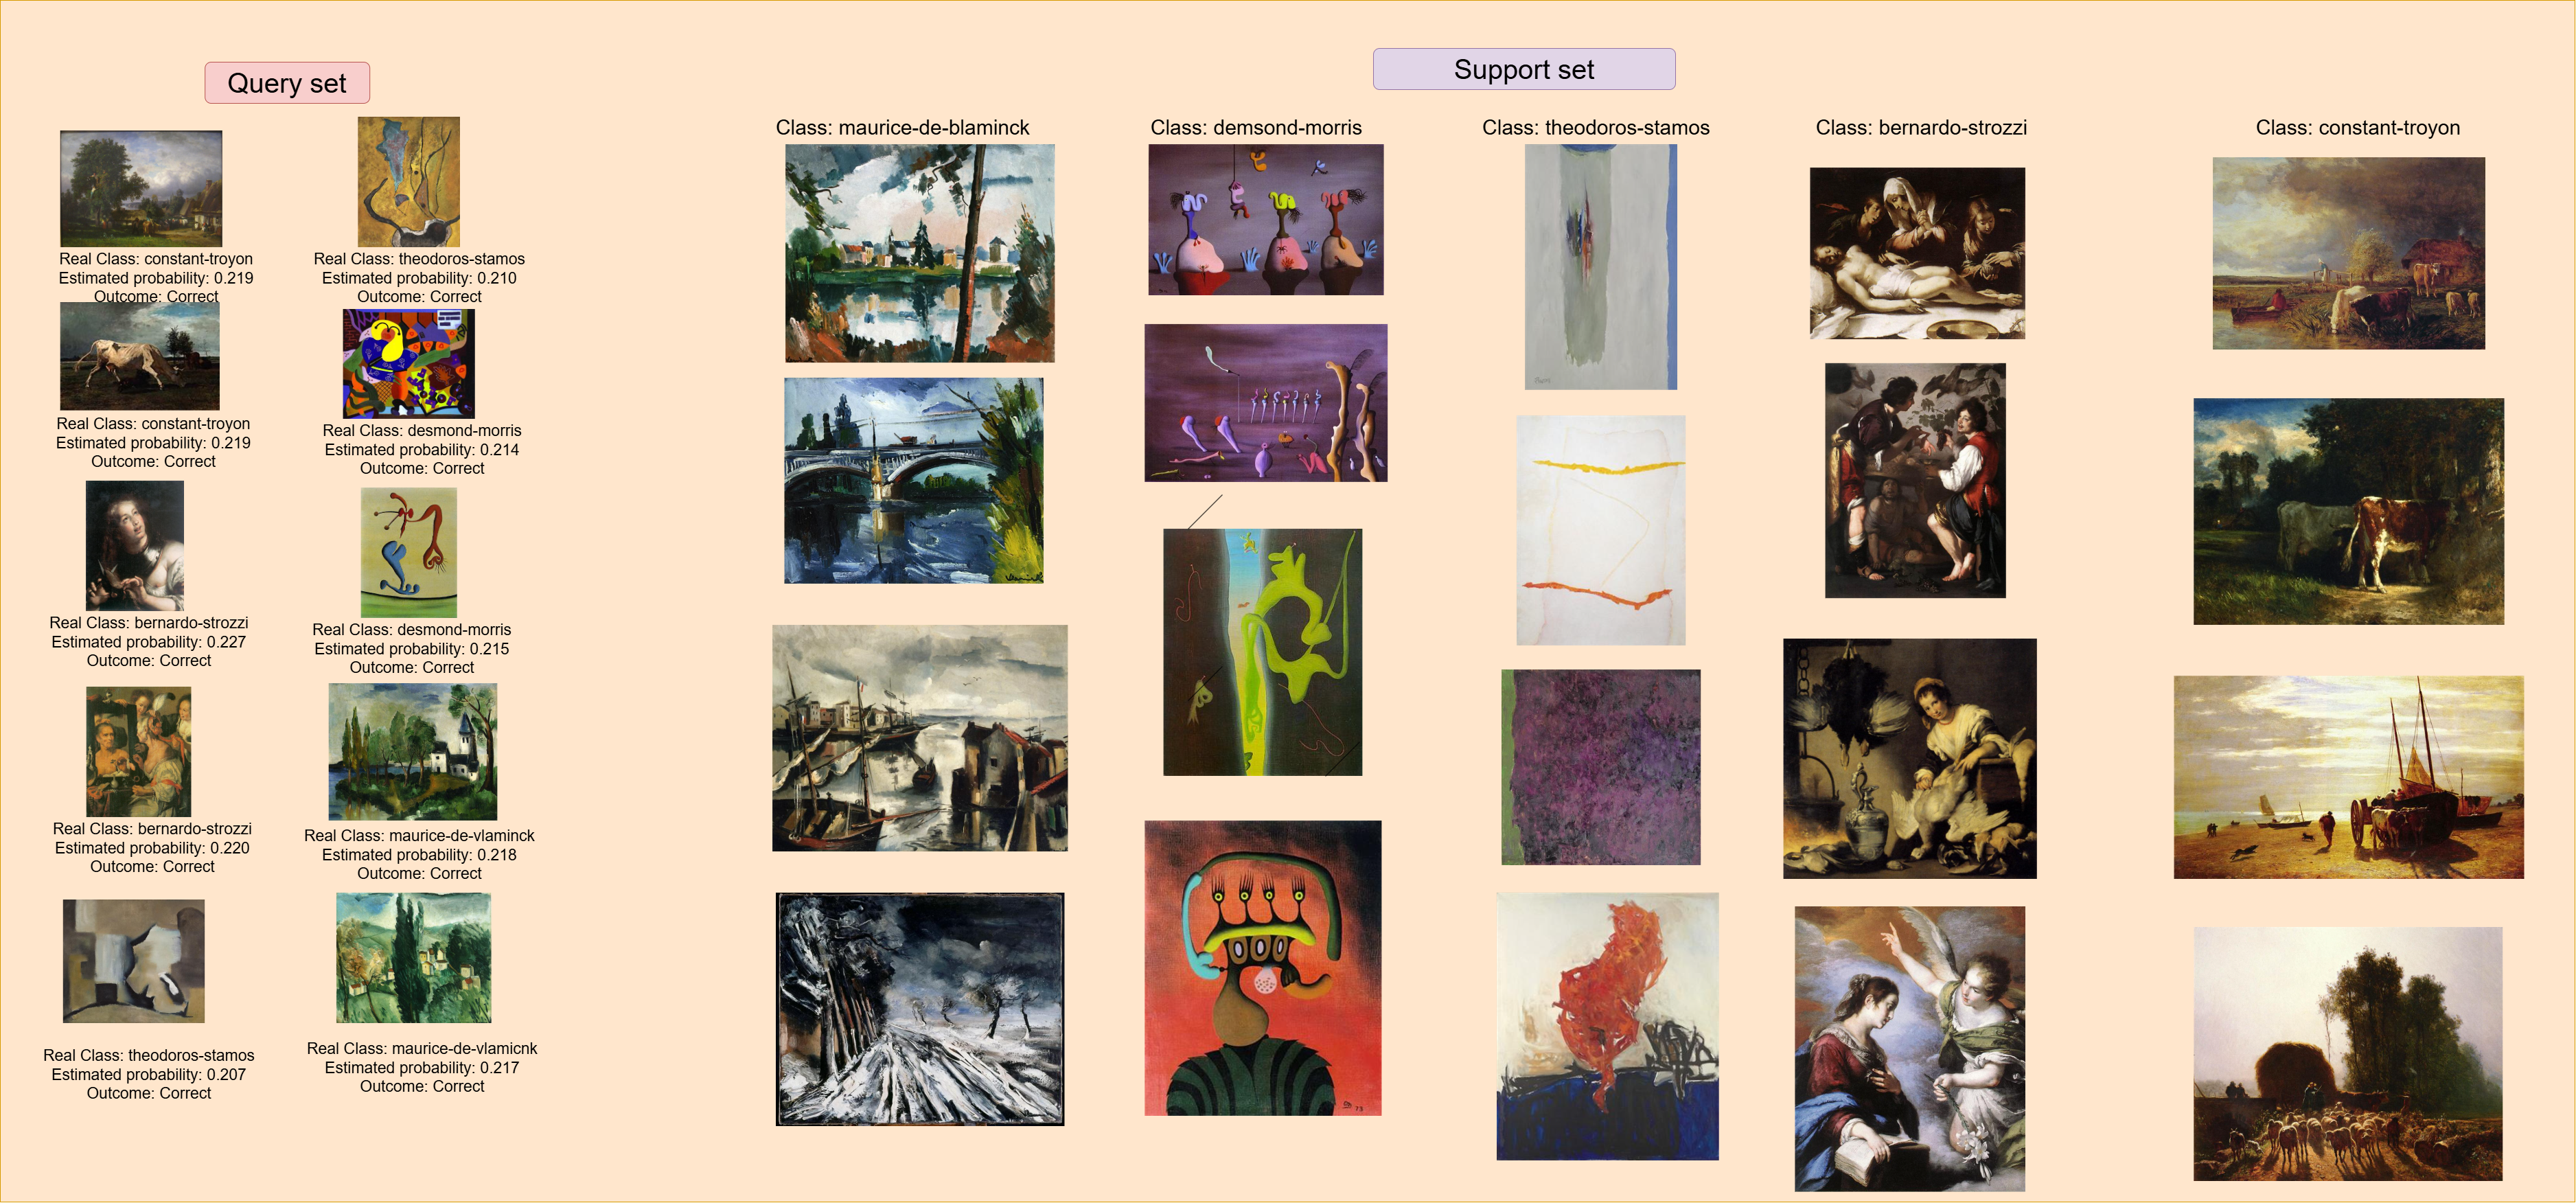
\includegraphics[width=\linewidth,height=0.35\textheight]{../img/episode_example.drawio.png}
    \caption{Example of a 5-Way 4-Shot Episode with 10 query}
\end{figure*}

\subsubsection{Experimental Protocol}

Our evaluation follows a standard few-shot learning protocol where each test episode represents an N-way classification task. For our artist classification domain:
\begin{itemize}
    \item \textbf{N-way Classification:} Each episode involves classifying among all available artist classes in our curated dataset subset
    \item \textbf{Support Set:} K examples per artist class are used to form class prototypes
    \item \textbf{Query Set:} Remaining examples serve as query instances for classification evaluation
\end{itemize}

We evaluate model performance across multiple shot settings to understand how the number of support examples affects classification accuracy: K ∈ \{1, 2, 4, 8, 16\} shots per class
\subsubsection{Statistical Robustness}

To ensure statistical validity and account for variance in few-shot performance, we implement a comprehensive multi-seed evaluation strategy:

Each experimental configuration is evaluated across 10 different random seeds: \{1, 2, 3, 4, 5, 6, 7, 8, 9, 42\}. This approach controls for:
\begin{itemize}
    \item \textbf{Support Set Sampling Variance:} Different random selections of K examples per class
    \item \textbf{Model Initialization Effects:} Stochastic components in model training and adaptation
    \item \textbf{Episode Construction Randomness:} Variation in query set composition across evaluation runs
\end{itemize}

\subsubsection{Baseline Methods}

We performe several experiments by changing the model used for the few-shot learning task and the backbone used for the CLIP model. The following models are used:
\begin{itemize}
    \item \textbf{CLIP + TIP-Adapter}: Standard CLIP model with TIP-Adapter \cite{TipAdapter} for few-shot adaptation
    \item \textbf{CLIP + APE}: Standard CLIP model with Adaptive Prior Refinement \cite{APE} for few-shot adaptation
    \item \textbf{CLIP + GDA-CLIP}: Standard CLIP model with Gradient-based Domain Adaptation \cite{GDA_CLIP} for few-shot adaptation
    \item \textbf{CLIP + TIMO}: Standard CLIP model with TIMO \cite{TIMO} for few-shot adaptation
    \item \textbf{CLIP + TIMO-S}: Our proposed StyCLIP model with integrated style-aware features
\end{itemize}

with the following backbones:
\begin{itemize}
    \item \textbf{CLIP RN50}: Standard CLIP model with ResNet-50 backbone
    \item \textbf{StyCLIP FLS1}: StyCLIP model with ResNet-50 backbone trained with 1-shot configuration
    \item \textbf{StyCLIP FLS4}: StyCLIP model with ResNet-50 backbone trained with 4-shot configuration
\end{itemize}

\subsubsection{Evaluation Metrics}

Performance assessment employs multiple complementary metrics to provide comprehensive evaluation: \textbf{Accuracy}, \textbf{Macro-averaged Precision}, \textbf{Macro-averaged Recall}, and \textbf{Macro-averaged F1-Score}. 

\section{Results}
\subsection{Hyperparameter Optimization Results}

The Optuna-based hyperparameter optimization process identified the optimal configurations for the two StyCLIP training scenarios.

For the FSL1 (1-shot) model, the best hyperparameters are:
\begin{itemize}
    \item Fusion Bottleneck Dimension: 64
    \item Learning Rate: 6.01 × 10\textsuperscript{-5}
    \item Dropout Rate: 0.0
    \item Weight Decay: 4.83 × 10\textsuperscript{-4}
    \item Validation Accuracy: 57.07\%
\end{itemize}

For the FSL4 (4-shot) model, the best hyperparameters are:
\begin{itemize}
    \item Fusion Bottleneck Dimension: 128
    \item Learning Rate: 1.02 × 10\textsuperscript{-5}
    \item Dropout Rate: 0.1
    \item Weight Decay: 1.03 × 10\textsuperscript{-6}
    \item Validation Accuracy: 60.53\%
\end{itemize}

\subsection{Evaluation Results}
The following tables present detailed performance metrics for all tested model-backbone combinations across 1-shot, 2-shot, 4-shot, 8-shot, and 16-shot scenarios. Here each results has been multiplied by 100 to express them as percentages.


\begin{table}[H]
\centering
\tiny
\caption{1-Shot Classification Results}
\label{tab:results_1shot}
\begin{tabular}{@{}lll*{4}{S[table-format=2.2]}@{}}
\toprule
\textbf{Model} & \textbf{Backbone} & \textbf{ACC} & \textbf{Precision} & \textbf{Recall} & \textbf{F1} \\
\midrule
APE & Custom\_FSL1\_RN50 & 2.05 & 0.93 & 2.05 & 0.87 \\
APE & Custom\_FSL4\_RN50 & 2.48 & 0.81 & 2.44 & 0.84 \\
APE & RN50 & 44.31 & 44.42 & 43.94 & 39.76 \\
GDA\_CLIP & Custom\_FSL1\_RN50 & 13.49 & 13.88 & 13.23 & 11.98 \\
GDA\_CLIP & Custom\_FSL4\_RN50 & 16.33 & 17.48 & 16.08 & 14.62 \\
GDA\_CLIP & RN50 & 41.41 & 38.86 & 40.76 & 35.33 \\
TIMO & Custom\_FSL1\_RN50 & 6.97 & 6.88 & 6.81 & 6.13 \\
TIMO & Custom\_FSL4\_RN50 & 7.37 & 7.57 & 7.17 & 6.69 \\
TIMO & RN50 & 43.88 & 44.32 & 43.52 & 40.29 \\
TIMO\_S & Custom\_FSL1\_RN50 & 7.28 & 7.27 & 7.11 & 6.38 \\
TIMO\_S & Custom\_FSL4\_RN50 & 7.31 & 7.56 & 7.13 & 6.63 \\
TIMO\_S & RN50 & \textbf{45.96} & \textbf{44.47} & \textbf{45.54} & \textbf{41.07} \\
Tip\_Adapter & Custom\_FSL1\_RN50 & 1.31 & 0.03 & 1.34 & 0.06 \\
Tip\_Adapter & Custom\_FSL4\_RN50 & 1.13 & 0.01 & 1.02 & 0.03 \\
Tip\_Adapter & RN50 & 38.65 & 30.85 & 38.38 & 30.92 \\
\bottomrule
\end{tabular}
\end{table}



\begin{table}[H]
\centering
\tiny
\caption{2-Shot Classification Results}
\label{tab:results_2shot}
\begin{tabular}{@{}lll*{4}{S[table-format=2.2]}@{}}
\toprule
\textbf{Model} & \textbf{Backbone} & \textbf{ACC} & \textbf{Precision} & \textbf{Recall} & \textbf{F1} \\
\midrule
APE & Custom\_FSL1\_RN50 & 3.55 & 1.51 & 3.51 & 1.51 \\
APE & Custom\_FSL4\_RN50 & 3.39 & 2.03 & 3.38 & 1.71 \\
APE & RN50 & 47.09 & 47.77 & 46.65 & 42.37 \\
GDA\_CLIP & Custom\_FSL1\_RN50 & 20.95 & 21.79 & 20.59 & 19.40 \\
GDA\_CLIP & Custom\_FSL4\_RN50 & 25.96 & 27.35 & 25.48 & 24.22 \\
GDA\_CLIP & RN50 & 47.22 & 47.90 & 46.41 & 42.47 \\
TIMO & Custom\_FSL1\_RN50 & 12.14 & 11.82 & 11.87 & 10.78 \\
TIMO & Custom\_FSL4\_RN50 & 13.55 & 13.67 & 13.21 & 12.16 \\
TIMO & RN50 & 47.89 & 48.43 & 47.32 & 43.72 \\
TIMO\_S & Custom\_FSL1\_RN50 & 13.76 & 13.84 & 13.45 & 12.44 \\
TIMO\_S & Custom\_FSL4\_RN50 & 15.38 & 15.69 & 15.02 & 13.92 \\
TIMO\_S & RN50 & \textbf{48.65} & \textbf{48.78} & \textbf{47.95} & \textbf{43.98} \\
Tip\_Adapter & Custom\_FSL1\_RN50 & 1.19 & 0.02 & 1.19 & 0.04 \\
Tip\_Adapter & Custom\_FSL4\_RN50 & 1.19 & 0.02 & 1.08 & 0.03 \\
Tip\_Adapter & RN50 & 40.73 & 32.99 & 40.33 & 32.58 \\
\bottomrule
\end{tabular}
\end{table}



\begin{table}[H]
\centering
\tiny
\caption{4-Shot Classification Results}
\label{tab:results_4shot}
\begin{tabular}{@{}lll*{4}{S[table-format=2.2]}@{}}
\toprule
\textbf{Model} & \textbf{Backbone} & \textbf{ACC} & \textbf{Precision} & \textbf{Recall} & \textbf{F1} \\
\midrule
APE & Custom\_FSL1\_RN50 & 4.62 & 2.09 & 4.42 & 2.17 \\
APE & Custom\_FSL4\_RN50 & 5.29 & 2.75 & 5.12 & 2.62 \\
APE & RN50 & 53.88 & 54.93 & 53.72 & 49.73 \\
GDA\_CLIP & Custom\_FSL1\_RN50 & 27.16 & 28.56 & 26.84 & 25.48 \\
GDA\_CLIP & Custom\_FSL4\_RN50 & 35.17 & 38.35 & 34.79 & 33.74 \\
GDA\_CLIP & RN50 & 55.54 & 58.24 & 54.97 & 52.66 \\
TIMO & Custom\_FSL1\_RN50 & 21.77 & 21.38 & 21.35 & 19.75 \\
TIMO & Custom\_FSL4\_RN50 & 23.43 & 25.00 & 23.06 & 22.13 \\
TIMO & RN50 & 56.48 & 59.14 & 55.90 & 53.96 \\
TIMO\_S & Custom\_FSL1\_RN50 & 23.24 & 23.04 & 22.81 & 21.19 \\
TIMO\_S & Custom\_FSL4\_RN50 & 26.36 & 28.69 & 25.97 & 25.27 \\
TIMO\_S & RN50 & \textbf{57.28} & \textbf{59.77} & \textbf{56.74} & \textbf{54.55} \\
Tip\_Adapter & Custom\_FSL1\_RN50 & 1.38 & 0.04 & 1.40 & 0.08 \\
Tip\_Adapter & Custom\_FSL4\_RN50 & 1.28 & 0.02 & 1.19 & 0.04 \\
Tip\_Adapter & RN50 & 44.95 & 39.16 & 44.38 & 37.19 \\
\bottomrule
\end{tabular}
\end{table}



\begin{table}[H]
\centering
\tiny
\caption{8-Shot Classification Results}
\label{tab:results_8shot}
\begin{tabular}{@{}lll*{4}{S[table-format=2.2]}@{}}
\toprule
\textbf{Model} & \textbf{Backbone} & \textbf{ACC} & \textbf{Precision} & \textbf{Recall} & \textbf{F1} \\
\midrule
APE & Custom\_FSL1\_RN50 & 5.35 & 2.57 & 5.27 & 2.57 \\
APE & Custom\_FSL4\_RN50 & 7.52 & 4.71 & 7.35 & 4.42 \\
APE & RN50 & 58.10 & 58.94 & 57.97 & 54.03 \\
GDA\_CLIP & Custom\_FSL1\_RN50 & 34.25 & 35.76 & 33.93 & 32.55 \\
GDA\_CLIP & Custom\_FSL4\_RN50 & 46.97 & 50.15 & 46.42 & 45.55 \\
GDA\_CLIP & RN50 & 63.61 & 67.18 & 63.19 & 61.57 \\
TIMO & Custom\_FSL1\_RN50 & 30.64 & 30.61 & 30.49 & 28.71 \\
TIMO & Custom\_FSL4\_RN50 & 38.38 & 40.46 & 37.90 & 36.52 \\
TIMO & RN50 & \textbf{65.26} & \textbf{68.43} & \textbf{64.93} & \textbf{63.66} \\
TIMO\_S & Custom\_FSL1\_RN50 & 32.17 & 33.14 & 31.92 & 30.49 \\
TIMO\_S & Custom\_FSL4\_RN50 & 40.89 & 43.57 & 40.41 & 39.13 \\
TIMO\_S & RN50 & 65.08 & 68.25 & 64.75 & 63.45 \\
Tip\_Adapter & Custom\_FSL1\_RN50 & 1.71 & 0.21 & 1.72 & 0.24 \\
Tip\_Adapter & Custom\_FSL4\_RN50 & 1.38 & 0.03 & 1.28 & 0.06 \\
Tip\_Adapter & RN50 & 48.44 & 45.26 & 47.99 & 41.20 \\
\bottomrule
\end{tabular}
\end{table}


\begin{table}[H]
\centering
\tiny
\caption{16-Shot Classification Results}
\label{tab:results_16shot}
\begin{tabular}{@{}lll*{4}{S[table-format=2.2]}@{}}
\toprule
\textbf{Model} & \textbf{Backbone} & \textbf{ACC} & \textbf{Precision} & \textbf{Recall} & \textbf{F1} \\
\midrule
APE & Custom\_FSL1\_RN50 & 6.73 & 3.35 & 6.55 & 3.37 \\
APE & Custom\_FSL4\_RN50 & 7.98 & 5.63 & 7.87 & 5.13 \\
APE & RN50 & 62.17 & 63.65 & 61.95 & 58.36 \\
GDA\_CLIP & Custom\_FSL1\_RN50 & 41.19 & 42.45 & 41.00 & 39.13 \\
GDA\_CLIP & Custom\_FSL4\_RN50 & 53.36 & 55.25 & 52.86 & 51.64 \\
GDA\_CLIP & RN50 & 73.06 & 76.12 & 72.58 & 71.63 \\
TIMO & Custom\_FSL1\_RN50 & 37.00 & 37.83 & 36.87 & 34.90 \\
TIMO & Custom\_FSL4\_RN50 & 43.27 & 45.16 & 42.80 & 41.36 \\
TIMO & RN50 & 73.36 & 76.59 & 72.94 & 72.09 \\
TIMO\_S & Custom\_FSL1\_RN50 & 39.20 & 40.52 & 39.01 & 37.22 \\
TIMO\_S & Custom\_FSL4\_RN50 & 48.75 & 50.58 & 48.27 & 46.90 \\
TIMO\_S & RN50 & \textbf{73.46} & \textbf{76.52} & \textbf{73.04} & \textbf{72.10} \\
Tip\_Adapter & Custom\_FSL1\_RN50 & 2.63 & 0.70 & 2.60 & 0.74 \\
Tip\_Adapter & Custom\_FSL4\_RN50 & 1.77 & 0.07 & 1.69 & 0.13 \\
Tip\_Adapter & RN50 & 52.91 & 51.90 & 52.37 & 46.38 \\
\bottomrule
\end{tabular}
\end{table}
\clearpage
\subsection{Statistical Analysis}


\begin{table}[H]
\centering
\tiny
\captionsetup{width=\linewidth, font=scriptsize, justification=centering}
\caption{Statistical Comparison Matrix for 1-Shot Classification (Accuracy \%). * indicates significant differences (p < 0.05) between models using paired t-tests.}
\label{tab:stats_1shot}
\resizebox{\textwidth}{!}{%
\begin{tabular}{@{}l*{15}{c}@{}}
\toprule
\rotatebox{90}{\textbf{Model}} & \rotatebox{90}{\textbf{APE\_FSL1}} & \rotatebox{90}{\textbf{APE\_FSL4}} & \rotatebox{90}{\textbf{APE\_RN50}} & \rotatebox{90}{\textbf{GDA\_FSL1}} & \rotatebox{90}{\textbf{GDA\_FSL4}} & \rotatebox{90}{\textbf{GDA\_RN50}} & \rotatebox{90}{\textbf{TIMO\_FSL1}} & \rotatebox{90}{\textbf{TIMO\_FSL4}} & \rotatebox{90}{\textbf{TIMO\_RN50}} & \rotatebox{90}{\textbf{TIMO\_S\_FSL1}} & \rotatebox{90}{\textbf{TIMO\_S\_FSL4}} & \rotatebox{90}{\textbf{TIMO\_S\_RN50}} & \rotatebox{90}{\textbf{Tip\_FSL1}} & \rotatebox{90}{\textbf{Tip\_FSL4}} & \rotatebox{90}{\textbf{Tip\_RN50}} \\
\midrule
APE\_FSL1 & 0.00 & -0.43 & -42.26* & -11.44* & -14.28* & -39.36* & -4.92* & -5.32* & -41.83* & -5.23* & -5.26* & -43.91* & 0.73 & 0.92* & -36.61* \\
APE\_FSL4 & 0.43 & 0.00 & -41.83* & -11.01* & -13.85* & -38.93* & -4.50* & -4.89* & -41.41* & -4.80* & -4.83* & -43.49* & 1.16* & 1.35* & -36.18* \\
APE\_RN50 & 42.26* & 41.83* & 0.00 & 30.83* & 27.98* & 2.91* & 37.34* & 36.94* & 0.43 & 37.03* & 37.00* & -1.65 & 43.00* & 43.18* & 5.66* \\
GDA\_FSL1 & 11.44* & 11.01* & -30.83* & 0.00 & -2.84* & -27.92* & 6.51* & 6.12* & -30.40* & 6.21* & 6.18* & -32.48* & 12.17* & 12.35* & -25.17* \\
GDA\_FSL4 & 14.28* & 13.85* & -27.98* & 2.84* & 0.00 & -25.08* & 9.36* & 8.96* & -27.55* & 9.05* & 9.02* & -29.63* & 15.02* & 15.20* & -22.32* \\
GDA\_RN50 & 39.36* & 38.93* & -2.91* & 27.92* & 25.08* & 0.00 & 34.43* & 34.04* & -2.48* & 34.13* & 34.10* & -4.56* & 40.09* & 40.28* & 2.75* \\
TIMO\_FSL1 & 4.92* & 4.50* & -37.34* & -6.51* & -9.36* & -34.43* & 0.00 & -0.40 & -36.91* & -0.31 & -0.34 & -38.99* & 5.66* & 5.84* & -31.68* \\
TIMO\_FSL4 & 5.32* & 4.89* & -36.94* & -6.12* & -8.96* & -34.04* & 0.40 & 0.00 & -36.51* & 0.09 & 0.06 & -38.59* & 6.06* & 6.24* & -31.28* \\
TIMO\_RN50 & 41.83* & 41.41* & -0.43 & 30.40* & 27.55* & 2.48* & 36.91* & 36.51* & 0.00 & 36.61* & 36.57* & -2.08 & 42.57* & 42.75* & 5.23* \\
TIMO\_S\_FSL1 & 5.23* & 4.80* & -37.03* & -6.21* & -9.05* & -34.13* & 0.31 & -0.09 & -36.61* & 0.00 & -0.03 & -38.69* & 5.96* & 6.15* & -31.38* \\
TIMO\_S\_FSL4 & 5.26* & 4.83* & -37.00* & -6.18* & -9.02* & -34.10* & 0.34 & -0.06 & -36.57* & 0.03 & 0.00 & -38.65* & 5.99* & 6.18* & -31.35* \\
TIMO\_S\_RN50 & 43.91* & 43.49* & 1.65 & 32.48* & 29.63* & 4.56* & 38.99* & 38.59* & 2.08 & 38.69* & 38.65* & 0.00 & 44.65* & 44.83* & 7.31* \\
Tip\_FSL1 & -0.73 & -1.16* & -43.00* & -12.17* & -15.02* & -40.09* & -5.66* & -6.06* & -42.57* & -5.96* & -5.99* & -44.65* & 0.00 & 0.18 & -37.34* \\
Tip\_FSL4 & -0.92* & -1.35* & -43.18* & -12.35* & -15.20* & -40.28* & -5.84* & -6.24* & -42.75* & -6.15* & -6.18* & -44.83* & -0.18 & 0.00 & -37.52* \\
Tip\_RN50 & 36.61* & 36.18* & -5.66* & 25.17* & 22.32* & -2.75* & 31.68* & 31.28* & -5.23* & 31.38* & 31.35* & -7.31* & 37.34* & 37.52* & 0.00 \\
\bottomrule
\end{tabular}%
}
\end{table}

\FloatBarrier



\begin{table}[H]
\centering
\tiny
\captionsetup{width=\linewidth, font=scriptsize, justification=centering}
\caption{Statistical Comparison Matrix for 2-Shot Classification (Accuracy \%). * indicates significant differences (p < 0.05) between models using paired t-tests.}
\label{tab:stats_2shot}
\resizebox{\textwidth}{!}{%
\begin{tabular}{@{}l*{15}{c}@{}}
\toprule
\rotatebox{90}{\textbf{Model}} & \rotatebox{90}{\textbf{APE\_FSL1}} & \rotatebox{90}{\textbf{APE\_FSL4}} & \rotatebox{90}{\textbf{APE\_RN50}} & \rotatebox{90}{\textbf{GDA\_FSL1}} & \rotatebox{90}{\textbf{GDA\_FSL4}} & \rotatebox{90}{\textbf{GDA\_RN50}} & \rotatebox{90}{\textbf{TIMO\_FSL1}} & \rotatebox{90}{\textbf{TIMO\_FSL4}} & \rotatebox{90}{\textbf{TIMO\_RN50}} & \rotatebox{90}{\textbf{TIMO\_S\_FSL1}} & \rotatebox{90}{\textbf{TIMO\_S\_FSL4}} & \rotatebox{90}{\textbf{TIMO\_S\_RN50}} & \rotatebox{90}{\textbf{Tip\_FSL1}} & \rotatebox{90}{\textbf{Tip\_FSL4}} & \rotatebox{90}{\textbf{Tip\_RN50}} \\
\midrule
APE\_FSL1 & 0.00 & 0.15 & -43.55* & -17.40* & -22.42* & -43.67* & -8.59* & -10.00* & -44.34* & -10.21* & -11.83* & -45.11* & 2.35* & 2.35* & -37.19* \\
APE\_FSL4 & -0.15 & 0.00 & -43.70* & -17.55* & -22.57* & -43.82* & -8.75* & -10.15* & -44.50* & -10.37* & -11.99* & -45.26* & 2.20* & 2.20* & -37.34* \\
APE\_RN50 & 43.55* & 43.70* & 0.00 & 26.15* & 21.13* & -0.12 & 34.95* & 33.55* & -0.80 & 33.33* & 31.71* & -1.56* & 45.90* & 45.90* & 6.36* \\
GDA\_FSL1 & 17.40* & 17.55* & -26.15* & 0.00 & -5.02* & -26.27* & 8.81* & 7.40* & -26.94* & 7.19* & 5.57* & -27.71* & 19.76* & 19.76* & -19.79* \\
GDA\_FSL4 & 22.42* & 22.57* & -21.13* & 5.02* & 0.00 & -21.25* & 13.82* & 12.42* & -21.93* & 12.20* & 10.58* & -22.69* & 24.77* & 24.77* & -14.77* \\
GDA\_RN50 & 43.67* & 43.82* & 0.12 & 26.27* & 21.25* & 0.00 & 35.08* & 33.67* & -0.67 & 33.46* & 31.83* & -1.44 & 46.02* & 46.02* & 6.48* \\
TIMO\_FSL1 & 8.59* & 8.75* & -34.95* & -8.81* & -13.82* & -35.08* & 0.00 & -1.41 & -35.75* & -1.62 & -3.24* & -36.51* & 10.95* & 10.95* & -28.59* \\
TIMO\_FSL4 & 10.00* & 10.15* & -33.55* & -7.40* & -12.42* & -33.67* & 1.41 & 0.00 & -34.34* & -0.21 & -1.83 & -35.11* & 12.35* & 12.35* & -27.19* \\
TIMO\_RN50 & 44.34* & 44.50* & 0.80 & 26.94* & 21.93* & 0.67 & 35.75* & 34.34* & 0.00 & 34.13* & 32.51* & -0.76 & 46.70* & 46.70* & 7.16* \\
TIMO\_S\_FSL1 & 10.21* & 10.37* & -33.33* & -7.19* & -12.20* & -33.46* & 1.62 & 0.21 & -34.13* & 0.00 & -1.62 & -34.89* & 12.57* & 12.57* & -26.97* \\
TIMO\_S\_FSL4 & 11.83* & 11.99* & -31.71* & -5.57* & -10.58* & -31.83* & 3.24* & 1.83 & -32.51* & 1.62 & 0.00 & -33.27* & 14.19* & 14.19* & -25.35* \\
TIMO\_S\_RN50 & 45.11* & 45.26* & 1.56* & 27.71* & 22.69* & 1.44 & 36.51* & 35.11* & 0.76 & 34.89* & 33.27* & 0.00 & 47.46* & 47.46* & 7.92* \\
Tip\_FSL1 & -2.35* & -2.20* & -45.90* & -19.76* & -24.77* & -46.02* & -10.95* & -12.35* & -46.70* & -12.57* & -14.19* & -47.46* & 0.00 & 0.00 & -39.54* \\
Tip\_FSL4 & -2.35* & -2.20* & -45.90* & -19.76* & -24.77* & -46.02* & -10.95* & -12.35* & -46.70* & -12.57* & -14.19* & -47.46* & -0.00 & 0.00 & -39.54* \\
Tip\_RN50 & 37.19* & 37.34* & -6.36* & 19.79* & 14.77* & -6.48* & 28.59* & 27.19* & -7.16* & 26.97* & 25.35* & -7.92* & 39.54* & 39.54* & 0.00 \\
\bottomrule
\end{tabular}%
}
\end{table}

\FloatBarrier



\begin{table}[H]
\centering
\tiny
\captionsetup{width=\linewidth, font=scriptsize, justification=centering}
\caption{Statistical Comparison Matrix for 4-Shot Classification (Accuracy \%). * indicates significant differences (p < 0.05) between models using paired t-tests.}
\label{tab:stats_4shot}
\resizebox{\textwidth}{!}{%
\begin{tabular}{@{}l*{15}{c}@{}}
\toprule
\rotatebox{90}{\textbf{Model}} & \rotatebox{90}{\textbf{APE\_FSL1}} & \rotatebox{90}{\textbf{APE\_FSL4}} & \rotatebox{90}{\textbf{APE\_RN50}} & \rotatebox{90}{\textbf{GDA\_FSL1}} & \rotatebox{90}{\textbf{GDA\_FSL4}} & \rotatebox{90}{\textbf{GDA\_RN50}} & \rotatebox{90}{\textbf{TIMO\_FSL1}} & \rotatebox{90}{\textbf{TIMO\_FSL4}} & \rotatebox{90}{\textbf{TIMO\_RN50}} & \rotatebox{90}{\textbf{TIMO\_S\_FSL1}} & \rotatebox{90}{\textbf{TIMO\_S\_FSL4}} & \rotatebox{90}{\textbf{TIMO\_S\_RN50}} & \rotatebox{90}{\textbf{Tip\_FSL1}} & \rotatebox{90}{\textbf{Tip\_FSL4}} & \rotatebox{90}{\textbf{Tip\_RN50}} \\
\midrule
APE\_FSL1 & 0.00 & -0.67 & -49.27* & -22.54* & -30.55* & -50.92* & -17.16* & -18.81* & -51.87* & -18.62* & -21.74* & -52.66* & 3.24* & 3.33* & -40.34* \\
APE\_FSL4 & 0.67 & 0.00 & -48.59* & -21.87* & -29.88* & -50.24* & -16.48* & -18.13* & -51.19* & -17.95* & -21.07* & -51.99* & 3.91* & 4.01* & -39.66* \\
APE\_RN50 & 49.27* & 48.59* & 0.00 & 26.73* & 18.72* & -1.65 & 32.11* & 30.46* & -2.60* & 30.64* & 27.52* & -3.39* & 52.51* & 52.60* & 8.93* \\
GDA\_FSL1 & 22.54* & 21.87* & -26.73* & 0.00 & -8.01* & -28.38* & 5.38* & 3.73* & -29.33* & 3.91* & 0.80 & -30.12* & 25.78* & 25.87* & -17.80* \\
GDA\_FSL4 & 30.55* & 29.88* & -18.72* & 8.01* & 0.00 & -20.37* & 13.39* & 11.74* & -21.31* & 11.93* & 8.81* & -22.11* & 33.79* & 33.88* & -9.79* \\
GDA\_RN50 & 50.92* & 50.24* & 1.65 & 28.38* & 20.37* & 0.00 & 33.76* & 32.11* & -0.95 & 32.29* & 29.17* & -1.74 & 54.16* & 54.25* & 10.58* \\
TIMO\_FSL1 & 17.16* & 16.48* & -32.11* & -5.38* & -13.39* & -34.76* & 0.00 & -1.65 & -34.71* & -1.47 & -4.59* & -35.50* & 20.40* & 20.49* & -23.18* \\
TIMO\_FSL4 & 18.81* & 18.13* & -30.46* & -3.73* & -11.74* & -32.11* & 1.65 & 0.00 & -33.06* & 0.18 & -2.94* & -33.85* & 22.05* & 22.14* & -21.53* \\
TIMO\_RN50 & 51.87* & 51.19* & 2.60* & 29.33* & 21.31* & 0.95 & 34.71* & 33.06* & 0.00 & 33.24* & 30.12* & -0.80 & 55.11* & 55.20* & 11.53* \\
TIMO\_S\_FSL1 & 18.62* & 17.95* & -30.64* & -3.91* & -11.93* & -32.29* & 1.47 & -0.18 & -34.13* & 0.00 & -3.12* & -34.04* & 21.87* & 21.96* & -21.71* \\
TIMO\_S\_FSL4 & 21.74* & 21.07* & -27.52* & -0.80 & -8.81* & -29.17* & 4.59* & 2.94* & -30.12* & 3.12 & 0.00 & -30.92* & 24.98* & 25.08* & -18.59* \\
TIMO\_S\_RN50 & 52.66* & 51.99* & 3.39* & 30.12* & 22.11* & 1.74 & 35.50* & 33.85* & 0.76 & 34.04* & 30.92* & 0.00 & 55.90* & 55.99* & 12.32* \\
Tip\_FSL1 & -3.24* & -3.91* & -52.51* & -25.78* & -33.79* & -54.16* & -20.40* & -22.05* & -55.11* & -21.87* & -24.98* & -55.90* & 0.00 & 0.09 & -43.58* \\
Tip\_FSL4 & -3.33* & -4.01* & -52.60* & -25.87* & -33.88* & -54.25* & -20.49* & -22.14* & -55.20* & -21.96* & -25.08* & -55.99* & -0.09 & 0.00 & -43.67* \\
Tip\_RN50 & 40.34* & 39.66* & -8.93* & 17.80* & 9.79* & -10.58* & 23.18* & 21.53* & -11.53* & 21.71* & 18.59* & -12.32* & 43.58* & 43.67* & 0.00 \\
\bottomrule
\end{tabular}%
}
\end{table}

\FloatBarrier
\clearpage

\begin{table}[H]
\centering
\tiny
\captionsetup{width=\linewidth, font=scriptsize, justification=centering}
\caption{Statistical Comparison Matrix for 8-Shot Classification (Accuracy \%) .* indicates significant differences (p < 0.05) between models using paired t-tests.}
\label{tab:stats_8shot}
\resizebox{\textwidth}{!}{%
\begin{tabular}{@{}l*{15}{c}@{}}
\toprule
\rotatebox{90}{\textbf{Model}} & \rotatebox{90}{\textbf{APE\_FSL1}} & \rotatebox{90}{\textbf{APE\_FSL4}} & \rotatebox{90}{\textbf{APE\_RN50}} & \rotatebox{90}{\textbf{GDA\_FSL1}} & \rotatebox{90}{\textbf{GDA\_FSL4}} & \rotatebox{90}{\textbf{GDA\_RN50}} & \rotatebox{90}{\textbf{TIMO\_FSL1}} & \rotatebox{90}{\textbf{TIMO\_FSL4}} & \rotatebox{90}{\textbf{TIMO\_RN50}} & \rotatebox{90}{\textbf{TIMO\_S\_FSL1}} & \rotatebox{90}{\textbf{TIMO\_S\_FSL4}} & \rotatebox{90}{\textbf{TIMO\_S\_RN50}} & \rotatebox{90}{\textbf{Tip\_FSL1}} & \rotatebox{90}{\textbf{Tip\_FSL4}} & \rotatebox{90}{\textbf{Tip\_RN50}} \\
\midrule
APE\_FSL1 & 0.00 & -2.17* & -52.75* & -28.90* & -41.62* & -58.26* & -25.29* & -33.03* & -59.91* & -26.82* & -35.54* & -59.72* & 3.64* & 3.98* & -43.09* \\
APE\_FSL4 & 2.17* & 0.00 & -50.58* & -26.73* & -39.45* & -56.09* & -23.12* & -30.86* & -57.74* & -24.65* & -33.36* & -57.55* & 5.81* & 6.15* & -40.92* \\
APE\_RN50 & 52.75* & 50.58* & 0.00 & 23.85* & 11.13* & -5.50* & 27.46* & 19.72* & -7.16* & 25.93* & 17.22* & -6.97* & 56.39* & 56.73* & 9.66* \\
GDA\_FSL1 & 34.46* & 33.21* & -20.98* & 0.00 & -12.17* & -31.87* & 4.19* & -2.08 & -32.17* & 1.99* & -7.55* & -32.26* & 38.56* & 39.42* & -11.71* \\
GDA\_FSL4 & 46.64* & 45.38* & -8.81* & 12.17* & 0.00 & -19.69* & 16.36* & 10.09* & -20.00* & 14.16* & 4.62* & -20.09* & 50.73* & 51.59* & 0.46 \\
GDA\_RN50 & 66.33* & 65.08* & 10.89* & 31.87* & 19.69* & 0.00 & 36.06* & 29.79* & -0.31 & 33.85* & 24.31* & -0.40 & 70.43* & 71.28* & 20.15* \\
TIMO\_FSL1 & 25.29* & 23.12* & -27.46* & -3.61* & -16.33* & -32.97* & 0.00 & -7.74* & -34.62* & -1.53 & -10.24* & -34.43* & 28.93* & 29.27* & -17.80* \\
TIMO\_FSL4 & 33.03* & 30.86* & -19.72* & 4.13* & -8.59* & -25.23* & 7.74* & 0.00 & -26.88* & 6.21* & -2.51 & -26.70* & 36.67* & 37.00* & -10.06* \\
TIMO\_RN50 & 59.91* & 57.74* & 7.16* & 31.01* & 18.29* & 1.65 & 34.62* & 26.88* & 0.00 & 33.09* & 24.37* & 0.18 & 63.55* & 63.88* & 16.82* \\
TIMO\_S\_FSL1 & 26.82* & 24.65* & -25.93* & -2.08 & -14.80* & -31.44* & 1.53 & -6.21* & -33.09* & 0.00 & -8.72* & -32.91* & 30.46* & 30.80* & -16.27* \\
TIMO\_S\_FSL4 & 35.54* & 33.36* & -17.22* & 6.64* & -6.09* & -22.72* & 10.24* & 2.51 & -24.37* & 8.72* & 0.00 & -24.19* & 39.17* & 39.51* & -7.55* \\
TIMO\_S\_RN50 & 59.72* & 57.55* & 6.97* & 30.83* & 18.10* & 1.47 & 34.43* & 26.70* & 0.09 & 34.25* & 24.71* & 0.00 & 70.83* & 71.68* & 20.55* \\
Tip\_FSL1 & -4.10* & -5.35* & -59.54* & -38.56* & -50.73* & -70.43* & -34.37* & -40.64* & -70.73* & -36.57* & -46.12* & -70.83* & 0.00 & 0.86 & -50.28* \\
Tip\_FSL4 & -4.95* & -6.21* & -60.40* & -39.42* & -51.59* & -71.28* & -35.23* & -41.50* & -71.59* & -37.43* & -46.97* & -71.68* & -0.86 & 0.00 & -51.13* \\
Tip\_RN50 & 46.18* & 44.92* & -9.27* & 11.71* & -0.46 & -20.15* & 15.90* & 9.63* & -20.46* & 13.70* & 4.16* & -20.55* & 50.28* & 51.13* & 0.00 \\
\bottomrule
\end{tabular}%
}
\end{table}

\FloatBarrier



\begin{table}[H]
\centering
\tiny
\captionsetup{width=\linewidth, font=scriptsize, justification=centering}
\caption{Statistical Comparison Matrix for 16-Shot Classification (Accuracy \%). * indicates significant differences (p < 0.05) between models using paired t-tests.}
\label{tab:stats_16shot}
\resizebox{\textwidth}{!}{%
\begin{tabular}{@{}l*{15}{c}@{}}
\toprule
\rotatebox{90}{\textbf{Model}} & \rotatebox{90}{\textbf{APE\_FSL1}} & \rotatebox{90}{\textbf{APE\_FSL4}} & \rotatebox{90}{\textbf{APE\_RN50}} & \rotatebox{90}{\textbf{GDA\_FSL1}} & \rotatebox{90}{\textbf{GDA\_FSL4}} & \rotatebox{90}{\textbf{GDA\_RN50}} & \rotatebox{90}{\textbf{TIMO\_FSL1}} & \rotatebox{90}{\textbf{TIMO\_FSL4}} & \rotatebox{90}{\textbf{TIMO\_RN50}} & \rotatebox{90}{\textbf{TIMO\_S\_FSL1}} & \rotatebox{90}{\textbf{TIMO\_S\_FSL4}} & \rotatebox{90}{\textbf{TIMO\_S\_RN50}} & \rotatebox{90}{\textbf{Tip\_FSL1}} & \rotatebox{90}{\textbf{Tip\_FSL4}} & \rotatebox{90}{\textbf{Tip\_RN50}} \\
\midrule
APE\_FSL1 & 0.00 & -1.25 & -55.44* & -34.46* & -46.64* & -66.33* & -30.28* & -36.54* & -66.64* & -32.48* & -42.02* & -66.73* & 4.10* & 4.95* & -46.18* \\
APE\_FSL4 & 1.25 & 0.00 & -54.19* & -33.21* & -45.38* & -65.08* & -29.02* & -35.29* & -65.38* & -31.22* & -40.76* & -65.47* & 5.35* & 6.21* & -44.92* \\
APE\_RN50 & 55.44* & 54.19* & 0.00 & 20.98* & 8.81* & -10.89* & 25.17* & 18.90* & -11.19* & 22.97* & 13.43* & -11.28* & 59.54* & 60.40* & 9.27* \\
GDA\_FSL1 & 34.46* & 33.21* & -20.98* & 0.00 & -12.17* & -31.87* & 4.19* & -2.08 & -32.17* & 1.99* & -7.55* & -32.26* & 38.56* & 39.42* & -11.71* \\
GDA\_FSL4 & 46.64* & 45.38* & -8.81* & 12.17* & 0.00 & -19.69* & 16.36* & 10.09* & -20.00* & 14.16* & 4.62* & -20.09* & 50.73* & 51.59* & 0.46 \\
GDA\_RN50 & 66.33* & 65.08* & 10.89* & 31.87* & 19.69* & 0.00 & 36.06* & 29.79* & -0.31 & 33.85* & 24.31* & -0.40 & 70.43* & 71.28* & 20.15* \\
TIMO\_FSL1 & 25.29* & 23.12* & -27.46* & -3.61* & -16.33* & -32.97* & 0.00 & -7.74* & -34.62* & -1.53 & -10.24* & -34.43* & 28.93* & 29.27* & -17.80* \\
TIMO\_FSL4 & 33.03* & 30.86* & -19.72* & 4.13* & -8.59* & -25.23* & 7.74* & 0.00 & -26.88* & 6.21* & -2.51 & -26.70* & 36.67* & 37.00* & -10.06* \\
TIMO\_RN50 & 59.91* & 57.74* & 7.16* & 31.01* & 18.29* & 1.65 & 34.62* & 26.88* & 0.00 & 33.09* & 24.37* & 0.18 & 63.55* & 63.88* & 16.82* \\
TIMO\_S\_FSL1 & 26.82* & 24.65* & -25.93* & -2.08 & -14.80* & -31.44* & 1.53 & -6.21* & -33.09* & 0.00 & -8.72* & -32.91* & 30.46* &  30.80* & -16.27* \\
TIMO\_S\_FSL4 & 35.54* & 33.36* & -17.22* & 6.64* & -6.09* & -22.72* & 10.24* & 2.51 & -24.37* & 8.72* & 0.00 & -24.19* & 39.17* & 39.51* & -7.55* \\
TIMO\_S\_RN50 & 59.72* & 57.55* & 6.97* & 30.83* & 18.10* & 1.47 & 34.43* & 26.70* & 0.09 & 34.25* & 24.71* & 0.00 & 70.83* & 71.68* & 20.55* \\
Tip\_FSL1 & -4.10* & -5.35* & -59.54* & -38.56* & -50.73* & -70.43* & -34.37* & -40.64* & -70.73* & -36.57* & -46.12* & -70.83* & 0.00 & 0.86 & -50.28* \\
Tip\_FSL4 & -4.95* & -6.21* & -60.40* & -39.42* & -51.59* & -71.28* & -35.23* & -41.50* & -71.59* & -37.43* & -46.97* & -71.68* & -0.86 & 0.00 & -51.13* \\
Tip\_RN50 & 46.18* & 44.92* & -9.27* & 11.71* & -0.46 & -20.15* & 15.90* & 9.63* & -20.46* & 13.70* & 4.16* & -20.55* & 50.28* & 51.13* & 0.00 \\
\bottomrule
\end{tabular}%
}
\end{table}

\FloatBarrier
\clearpage

\subsection{Discussion}


Our comprehensive evaluation of StyCLIP reveals that integrating explicit style-aware features does not improve few-shot artist classification performance. 

Standard CLIP with RN50 backbone consistently outperforms both StyCLIP variants across all shot configurations. In 16-shot scenarios, standard CLIP achieves 73.46\% accuracy while the best StyCLIP variant reaches only 48.75\%—a statistically significant 25 percentage point difference. Among few-shot methods, TIMO and TIMO\_S demonstrate superior performance, with no significant differences between them when using standard RN50.

Classification accuracy improves substantially with more support examples (TIMO\_S: 45.96\% to 73.46\% from 1-shot to 16-shot). However, both StyCLIP variants consistently underperform across all conditions, suggesting that explicit Gram matrix-based style modeling may interfere with pre-trained semantic representations rather than enhance them.

The experimental results reveal several key insights across different shot configurations. In 1-shot scenarios with extremely limited data, CLIP-based models with RN50 backbone (particularly TIMO and TIMO\_S) achieve significantly superior results compared to StyCLIP variants and other methods. The performance of approaches that explicitly integrate stylistic components remains substantially lower, suggesting that adding these features does not aid generalization under minimal data conditions.

As the number of support examples increases to 2-shot and 4-shot, all models show performance improvements, but the gap between standard CLIP RN50 and StyCLIP versions remains pronounced. Standard models continue to dominate, while solutions with custom backbones struggle to exceed 25\% accuracy in lower-shot scenarios.

In higher-shot configurations (8-shot and 16-shot), while performance differences between models decrease slightly, CLIP RN50 and TIMO\_S remain the most effective, achieving over 73\% accuracy in 16-shot cases. StyCLIP versions fail to bridge this performance gap, confirming that explicit integration of style information through Gram matrices does not provide concrete benefits for few-shot artist classification.



\section{Conclusion}

Our results indicate that CLIP's pre-trained features already capture sufficient stylistic information for artist classification. The negative results highlight the complexity of effectively integrating style transfer techniques into foundation models without disrupting learned semantic-visual alignment.
Alternative approaches such as attention-based style integration or domain-specific fine-tuning without architectural modifications may prove more effective than explicit style modeling for artistic classification tasks.

\section{Acknowledgments}
This work was proposed by PhD student \textbf{Nicola Fanelli} and \textbf{Prof. Giovanna Castellano} at the University of Bari. 
\clearpage
\bibliographystyle{IEEEtran}
\bibliography{bibo}

\end{document}